% !TEX root = ../my-thesis.tex
%
% ------------------------------------  --> cover title page
\begin{titlepage}
	\pdfbookmark[0]{Cover}{Cover}
	\flushright
	\hfill
	\vfill

  \begin{figure}[htb]
  \centering
  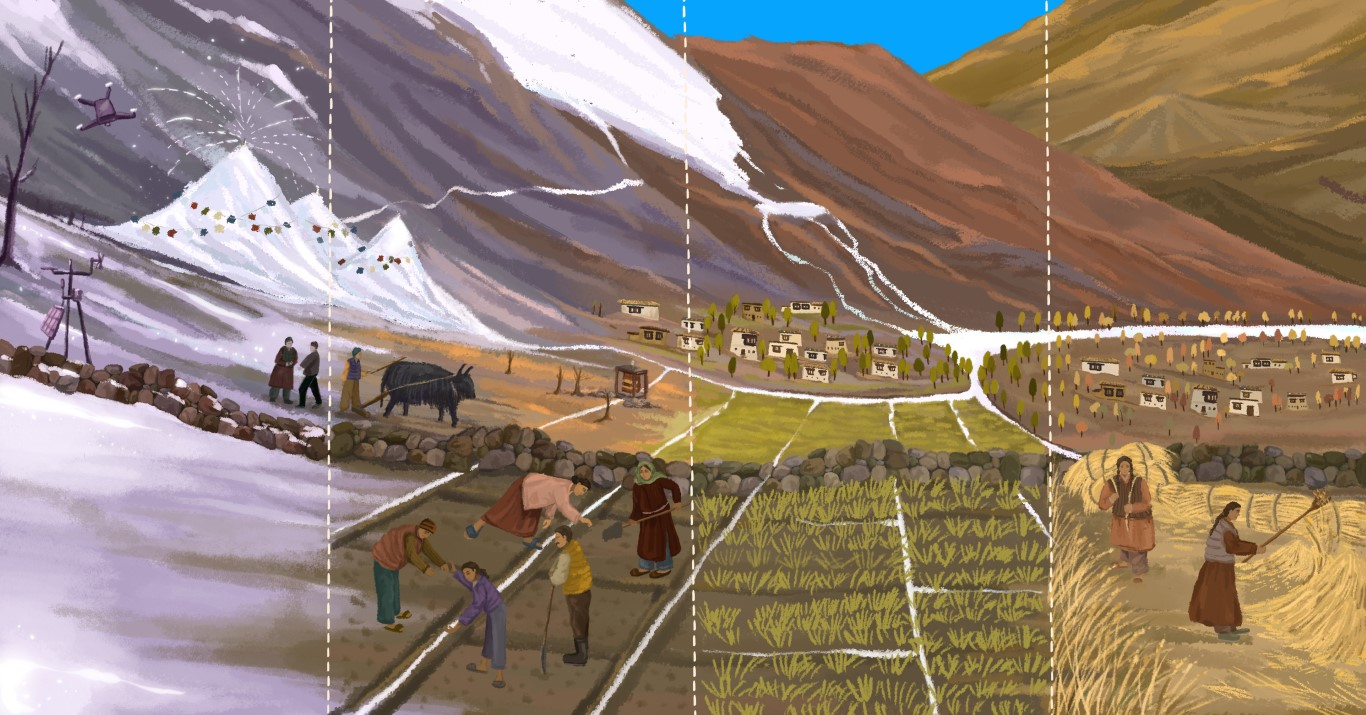
\includegraphics[width=\textwidth]{figs/Illustration.jpg}
  \end{figure}
	{\Large\thesisTitle \par}
	\rule[5pt]{\textwidth}{.4pt} \par
	{\large\thesisName}
	\vfill
	\textit{\large\thesisDate} \\
	% Version \thesisVersion
\end{titlepage}


% ------------------------------------  --> main title page
\begin{titlepage}
	\pdfbookmark[0]{Titlepage}{Titlepage}
	\tgherosfont
	\centering

	% {\Large \thesisUniversity} \\[4mm]
	
\includegraphics[width=6cm]{figs/unifr-logo} \\[2mm]
	\textsf{\thesisUniversityDepartment} \\
	% \textsf{\thesisUniversityInstitute} \\
	\textsf{\thesisUniversityGroup} \\

	\vfill
	\includegraphics[width=3cm]{figs/air_logo_circle} \\[2mm]
	% {\large \thesisSubject} \\[5mm]
	{\LARGE \color{ctcolortitle}\textbf{\thesisTitle} \\[10mm]}
	{\Large \thesisName} \\

	\vfill
	% \begin{minipage}[t]{.27\textwidth}
	% 	\raggedleft
	% 	\textit{1. Reviewer}
	% \end{minipage}
	% \hspace*{15pt}
	% \begin{minipage}[t]{.65\textwidth}
	% 	{\Large \thesisFirstReviewer} \\
	%   	% {\small \thesisFirstReviewerDepartment} \\[-1mm]
	% 	{\small \thesisFirstReviewerUniversity}
	% \end{minipage} \\[5mm]
	% \begin{minipage}[t]{.27\textwidth}
	% 	\raggedleft
	% 	\textit{2. Reviewer}
	% \end{minipage}
	% \hspace*{15pt}
	% \begin{minipage}[t]{.65\textwidth}
	% 	{\Large \thesisSecondReviewer} \\
	%   	% {\small \thesisSecondReviewerDepartment} \\[-1mm]
	% 	{\small \thesisSecondReviewerUniversity}
	% \end{minipage} \\[10mm]
	% \begin{minipage}[t]{.27\textwidth}
	% 	\raggedleft
	% 	\textit{3. Reviewer}
	% \end{minipage}
	% \hspace*{15pt}
	% \begin{minipage}[t]{.65\textwidth}
	% 	{\Large \thesisThirdReviewer} \\
	%   	% {\small \thesisThirdReviewerDepartment} \\[-1mm]
	% 	{\small \thesisThirdReviewerUniversity}
	% \end{minipage} \\[10mm]
	% \begin{minipage}[t]{.27\textwidth}
	% 	\raggedleft
	% 	\textit{4. Reviewer}
	% \end{minipage}
	% \hspace*{15pt}
	% \begin{minipage}[t]{.65\textwidth}
	% 	{\Large \thesisFourthReviewer} \\
	%   	% {\small \thesisFourthReviewerDepartment} \\[-1mm]
	% 	{\small \thesisFourthReviewerUniversity}
	% \end{minipage} \\[10mm]
	% \begin{minipage}[t]{.27\textwidth}
	% 	\raggedleft
	% 	\textit{Supervisor}
	% \end{minipage}
	% \hspace*{15pt}
	% \begin{minipage}[t]{.65\textwidth}
	% 	\thesisFirstSupervisor\
	% \end{minipage} \\[10mm]
	\begin{minipage}[t]{.27\textwidth}
		\raggedleft
		\textit{Supervisor}
	\end{minipage}
	\hspace*{15pt}
	\begin{minipage}[t]{.65\textwidth}
		{\Large \thesisFirstSupervisor} \\
	\end{minipage} \\[10mm]

	% \thesisDate \\

\end{titlepage}


% ------------------------------------  --> lower title back for single page layout

This thesis was presented to the Faculty of Science of the University of Fribourg (Switzerland) in consideration
for the award of \textit{Doctor rerum naturalium} on \thesisDate.

\vfill
{\large \textbf{Citation} \\}
Balasubramanian, S. \thesisTitle . \thesisUniversityGroup, 2022.

\hfill
\vfill
{
	\small
	\textbf{\thesisName} \\
	\textit{\thesisTitle} \\
	\thesisSubject, \thesisDate \\
	Reviewers: \thesisFirstReviewer,\ \thesisSecondReviewer,\ \thesisThirdReviewer\ and \thesisFourthReviewer \\
	Supervisor: \thesisFirstSupervisor \\
	English editors: Lou Del Bello\ and Ana Rodríguez Crespo\\[1.5em]
	\textbf{\thesisUniversity} \\
	\textit{\thesisUniversityGroup} \\
	% \thesisUniversityInstitute \\
	\thesisUniversityDepartment \\
	\thesisUniversityStreetAddress \\
	\thesisUniversityCity \\
	\thesisUniversityPostalCode \\
  \url{https://www.unifr.ch/geo/cryosphere/en/}\\
\\
  This thesis was typeset with \LaTeXe.
  It uses the \textit{Clean Thesis} style developed by Ricardo Langner.
  Download the \textit{Clean Thesis} style at \url{http://cleanthesis.der-ric.de/}.

  On the cover: Composite image of four different seasons, farming cycles and the role water plays through its
  changing states in an arid mountain catchment. From left to right: The artificial ice reservoir construction and
  measurement campaigns using fountains, drones, and automatic weather stations during the winter season; flood
  irrigation of the farm in the spring season; the cultivated plantations in the summer season; harvesting the
  plantations in the autumn season.

  Correspondence to Suryanarayanan Balasubramanian (gayashiva91@gmail.com).
}

